\subsection{Fremdrift og Styrtøj}

For at kunne styre bilens fremdrift og retning er bilen blevet udstyret med en H-bro\cite{lib:wikiHbro} og en RC hobby servomotor\cite{lib:wiki-RC-Servo}.
H-broen styrer bilens motor ved hjælp af et PWM signal og 2 digitale signaler fra Pi kontrolleren. 
Hjertet i H-broen er L298N\cite{lib:L298N_datablad}, som er en Fuld H-Bro motor controller. 
Den bestemmer med de to digitale signaler om motoren skal få bilen til at kører frem eller tilbage. 
PWM signalet bestemmer hvor stærkt bilen kører. 
L298N giver også mulighed for at bremse bilen.

Det er valgt selv at design et motorstyringsprint ud fra designanbefalingerne for L298N  i Multisim og Ultiboard og med henblik på at reducere elektromagnetisk støj mest muligt.

På samme måde som bilens motor bliver bilens styretøj også styret af et PWM til servomotoren. 
Servoens udslag til siderne bliver kontrolleret ved at lave et PWM signal med en pulsbredde mellem 0.5ms og 2.5ms. 
Det giver fuldt udslag til henholdsvis venstre og højre på ca. 40\si{\degree} til hver side.
Det var oprindeligt tiltænkt at begge PWM signaler skulle styres af det indbyggede PWM på Pi. 
Men det viste sig ikke muligt da det kun var muligt at sætte én PWM frekvens for begge PWM udgange. 
Derfor bliver motorens PWM, der er 40kHz, styret af hardwaren. 
Mens servoens PWM, der er ca. 50Hz, styret af en software PWM. 
Det er valgt for at belaste Pi'ens cpu mindst muligt.
For at de logiske signaler fra Pi'en til servo passer sammen er der designet et lille converter print der hæver signalet fra 3.3V til 5V.
\clearpage

\begin{figure}[h]
	\centering
	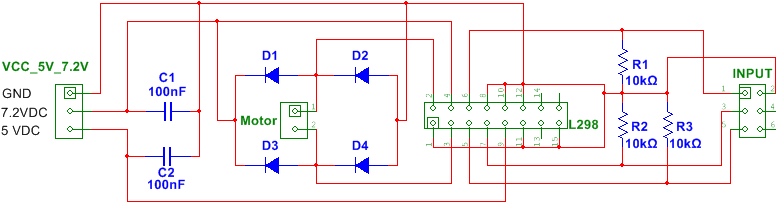
\includegraphics[width=\textwidth* 9/10]{../fig/billeder/MultiSim_H_Bro}
	\label{fig:MultiSim_HBro}
	\caption{MultiSim H-Bro}
\end{figure}

\begin{figure}[h]
	\centering
	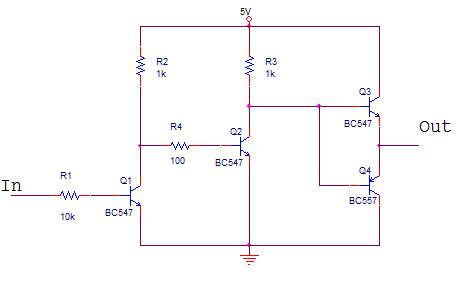
\includegraphics[width=\textwidth* 6/10]{../fig/billeder/servo_stepup}
	\caption{Diagram af signal converter}
	\label{fig:signal_converter}
\end{figure}
